\documentclass{article}

\usepackage[latin1]{inputenc}
\usepackage{tikz}
\usetikzlibrary{calc}
\usepackage{tkz-euclide}
\tikzset{line/.style={draw, thick, -latex'}}
%\usetikzlibrary{shapes,arrows}
\begin{document}
\pagestyle{empty}


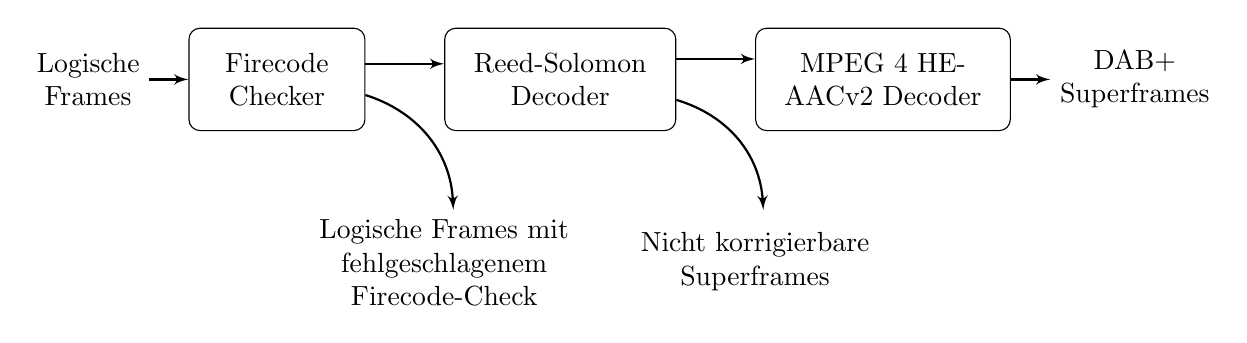
\begin{tikzpicture}[node distance = 1cm, auto]
\tikzstyle{block} = [rectangle, rounded corners, draw, text width=6em, text centered, minimum height=1.3cm]
\tikzstyle{Text} = [rectangle, rounded corners, text width=6em, text centered, minimum height=1.3cm]
\tikzstyle{rect} = [rectangle, draw, text width=9em, text centered, minimum height=2em]
\tikzstyle{input} = [rectangle, text width=2em, align=right, minimum height=3cm]

\node [block, text width=2.0cm](fire){Firecode Checker};
\node [Text, left=0.5cm of fire, text width=1.3cm, anchor=east](log){Logische Frames};
\node [block, right=1cm of fire, text width=2.7cm](rs){Reed-Solomon Decoder};
\node [block, right=1cm of rs, text width=3cm](mp4){MPEG 4 HE-AACv2 Decoder};
\node [Text, right=0.5cm of mp4, text width=1.9cm](super){DAB+ Superframes};
\node [Text, below=1cm of rs.south west, text width=3.3cm](n1){Logische Frames mit fehlgeschlagenem Firecode-Check};
\node [Text, below=1cm of mp4.south west, text width=3.3cm](n2){Nicht korrigierbare Superframes};


\path [line] (fire.10) -- (rs.170|-fire.10);
\path [line] (rs.10) -- (mp4.170|-rs.10);
\path [line] (mp4) -- (super);
\draw [line] (fire.350) to [bend left=35] (n1);
\draw [line] (rs.350) to [bend left=35] (n2);
\draw [line] (log) -- (fire);


\end{tikzpicture}
\end{document}